\begin{figure}[!ht]
 \begin{center}
  \scalebox{0.55}
  {
   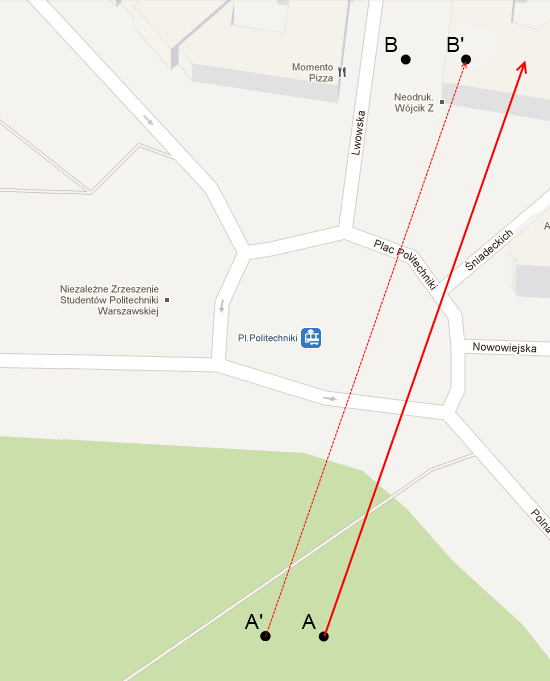
\includegraphics{figures/positionTracking.png}
  }
 \end{center}
 \caption{
  Pesymistyczny przykład konsekwencji błędu odczytu pozycji.
  Linią przerywaną zaznaczono wynik dokonanego odczytu, a linią ciagłą - to, jak wynik zostanie zinterpretowany przez użytkownika.
  [Źródło mapy: https://maps.google.pl/]
 }
 \label{fig:positionTracking}
\end{figure}
